% Options for packages loaded elsewhere
\PassOptionsToPackage{unicode}{hyperref}
\PassOptionsToPackage{hyphens}{url}
%
\documentclass[
]{article}
\usepackage{amsmath,amssymb}
\usepackage{lmodern}
\usepackage{iftex}
\ifPDFTeX
  \usepackage[T1]{fontenc}
  \usepackage[utf8]{inputenc}
  \usepackage{textcomp} % provide euro and other symbols
\else % if luatex or xetex
  \usepackage{unicode-math}
  \defaultfontfeatures{Scale=MatchLowercase}
  \defaultfontfeatures[\rmfamily]{Ligatures=TeX,Scale=1}
\fi
% Use upquote if available, for straight quotes in verbatim environments
\IfFileExists{upquote.sty}{\usepackage{upquote}}{}
\IfFileExists{microtype.sty}{% use microtype if available
  \usepackage[]{microtype}
  \UseMicrotypeSet[protrusion]{basicmath} % disable protrusion for tt fonts
}{}
\makeatletter
\@ifundefined{KOMAClassName}{% if non-KOMA class
  \IfFileExists{parskip.sty}{%
    \usepackage{parskip}
  }{% else
    \setlength{\parindent}{0pt}
    \setlength{\parskip}{6pt plus 2pt minus 1pt}}
}{% if KOMA class
  \KOMAoptions{parskip=half}}
\makeatother
\usepackage{xcolor}
\usepackage[margin=1in]{geometry}
\usepackage{longtable,booktabs,array}
\usepackage{calc} % for calculating minipage widths
% Correct order of tables after \paragraph or \subparagraph
\usepackage{etoolbox}
\makeatletter
\patchcmd\longtable{\par}{\if@noskipsec\mbox{}\fi\par}{}{}
\makeatother
% Allow footnotes in longtable head/foot
\IfFileExists{footnotehyper.sty}{\usepackage{footnotehyper}}{\usepackage{footnote}}
\makesavenoteenv{longtable}
\usepackage{graphicx}
\makeatletter
\def\maxwidth{\ifdim\Gin@nat@width>\linewidth\linewidth\else\Gin@nat@width\fi}
\def\maxheight{\ifdim\Gin@nat@height>\textheight\textheight\else\Gin@nat@height\fi}
\makeatother
% Scale images if necessary, so that they will not overflow the page
% margins by default, and it is still possible to overwrite the defaults
% using explicit options in \includegraphics[width, height, ...]{}
\setkeys{Gin}{width=\maxwidth,height=\maxheight,keepaspectratio}
% Set default figure placement to htbp
\makeatletter
\def\fps@figure{htbp}
\makeatother
\setlength{\emergencystretch}{3em} % prevent overfull lines
\providecommand{\tightlist}{%
  \setlength{\itemsep}{0pt}\setlength{\parskip}{0pt}}
\setcounter{secnumdepth}{5}
\usepackage{hyperref}
\hypersetup{
    colorlinks,
    linkcolor={blue!100!black},
    citecolor={blue!100!black},
    urlcolor={blue!100!black}
}
\usepackage{apacite}
\usepackage[round]{natbib} 
\usepackage{graphicx}
\usepackage{float}
\usepackage{caption}
\usepackage[toc,page]{appendix}
\usepackage{booktabs,caption}
\usepackage[flushleft]{threeparttable}
\usepackage{tabularx}
\usepackage{amsfonts}
\usepackage{amsmath}
\usepackage{xcolor}
\usepackage{scrextend}
\deffootnote[2em]{2em}{1em}{\textsuperscript{\thefootnotemark}\,}
\newcolumntype{Y}{>{\centering\arraybackslash}X}
%\usepackage[a4paper]{geometry}
\usepackage{caption}
\usepackage[bottom,flushmargin,hang,multiple]{footmisc}
\usepackage{pdflscape}
\usepackage[paper=portrait,pagesize]{typearea}
\usepackage{rotating}
\usepackage{fullpage}
\usepackage{tabu}
\ifLuaTeX
  \usepackage{selnolig}  % disable illegal ligatures
\fi
\usepackage[round]{natbib}
\bibliographystyle{sarb.bst}
\IfFileExists{bookmark.sty}{\usepackage{bookmark}}{\usepackage{hyperref}}
\IfFileExists{xurl.sty}{\usepackage{xurl}}{} % add URL line breaks if available
\urlstyle{same} % disable monospaced font for URLs
\hypersetup{
  hidelinks,
  pdfcreator={LaTeX via pandoc}}

\author{}
\date{\vspace{-2.5em}}

\begin{document}


\title{Basel III and the supply of bank credit in South Africa}


\author { 
Alister Milner\footnote{Loughborough University,School of Business and Economics,United Kingdom; Email: A.K.L.Milne@lboro.ac.uk}  \,\, 
Xolani Sibande\footnote{South African Reserve Bank, South Africa; Email: xolani.sibande@resbank.co.za}
}
\date{\today}
\maketitle

\begin{abstract}


\end{abstract}

\noindent\textbf{Keywords}: Bank capital, Bank regulation, Credit   \\
\textbf{JEL Codes}: G01, G18, G28, G32, G38
\newpage

\hypertarget{introduction}{%
\section{Introduction}\label{introduction}}

The paper investigates the impact of Basel III regulation on bank lending in South Africa. This introduction is an overview of the paper

\hypertarget{context}{%
\section{Context}\label{context}}

A review of policy context, with focus on South Africa but also reference to other emerging markets. Further detail in Appendix 1 and 2a.

\hypertarget{literature}{%
\section{Literature}\label{literature}}

\citet{osborne2017good}

\citet{jokipii2008cyclical}

\citet{gambacorta2004does}

\citet{schwert2018bank}

\citet{kim2017effect}

\citet{carlson2013capital}

\citet{tabak2011bank}

\citet{altunbas2004bank}

\citet{gambacorta2018bank}

\citet{berrospide2010effects}

\newpage

\hypertarget{developments-in-south-african-banking}{%
\section{Developments in South African Banking}\label{developments-in-south-african-banking}}

\begin{figure}[H]

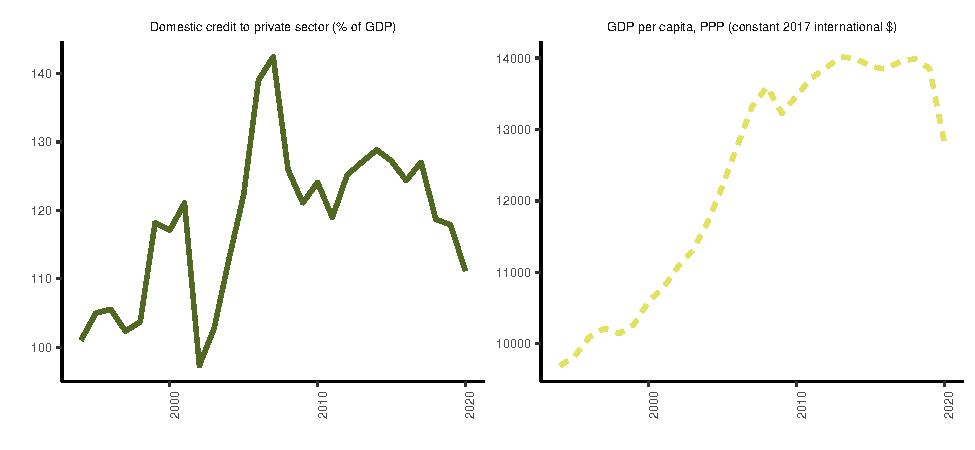
\includegraphics{Bank_capital_and_bank_lending_files/figure-latex/unnamed-chunk-1-1} \hfill{}

\caption{Credit Cycle. Source: South African Reserve Bank (2022)}\label{fig:unnamed-chunk-1}
\end{figure}

\begin{figure}[H]

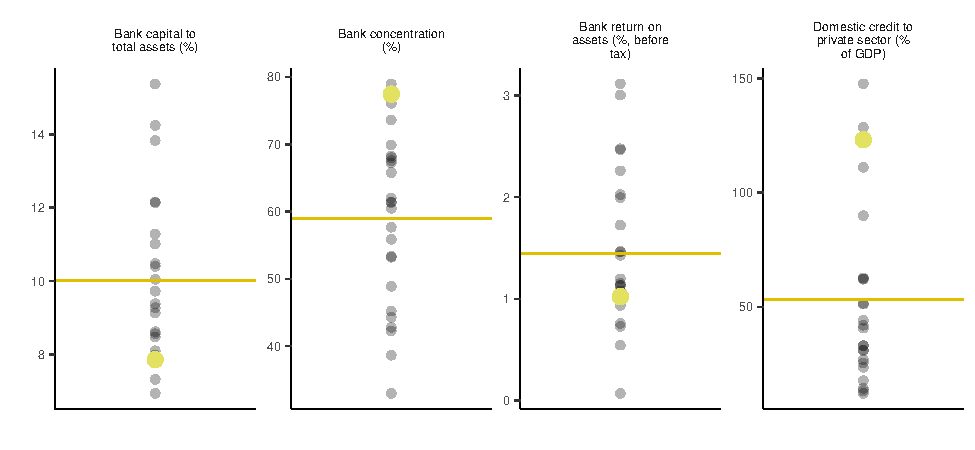
\includegraphics{Bank_capital_and_bank_lending_files/figure-latex/unnamed-chunk-2-1} \hfill{}

\caption{Capital Buffers. Source: South African Reserve Bank (2022)}\label{fig:unnamed-chunk-2}
\end{figure}

\begin{figure}[H]

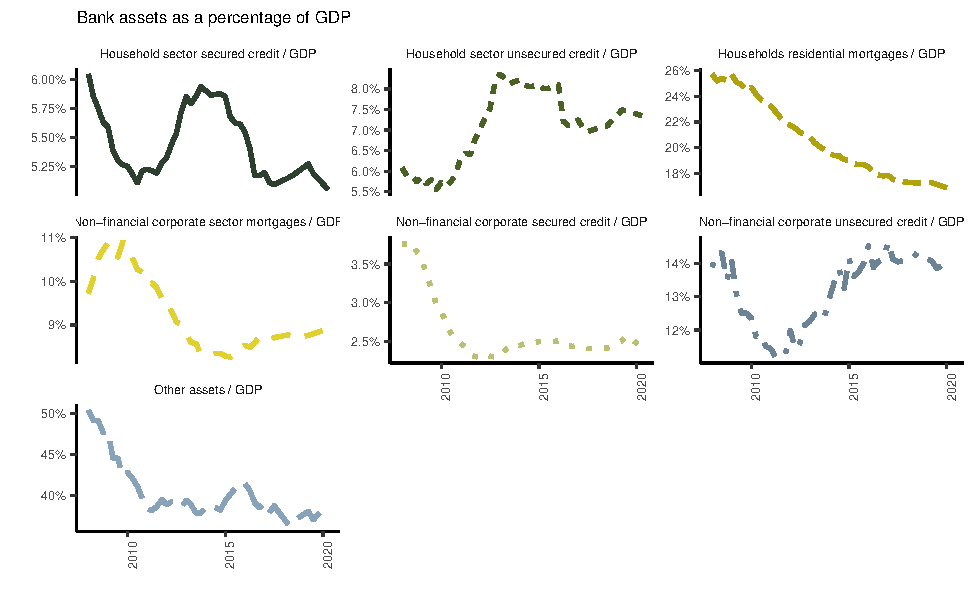
\includegraphics{Bank_capital_and_bank_lending_files/figure-latex/unnamed-chunk-5-1} \hfill{}

\caption{Bank assets. Source: South African Reserve Bank (2022)}\label{fig:unnamed-chunk-5}
\end{figure}

\begin{figure}[H]

\includegraphics{Bank_capital_and_bank_lending_files/figure-latex/unnamed-chunk-6-1} \hfill{}

\caption{Lending Rates. Source: South African Reserve Bank (2022)}\label{fig:unnamed-chunk-6}
\end{figure}

\hypertarget{specification}{%
\section{Specification}\label{specification}}

\hypertarget{estimation-results}{%
\section{Estimation Results}\label{estimation-results}}

\hypertarget{conclusion}{%
\section{Conclusion}\label{conclusion}}

\newpage

\hypertarget{appendix-descriptive-analysis}{%
\section{Appendix: Descriptive Analysis}\label{appendix-descriptive-analysis}}

\hypertarget{data}{%
\subsection{Data}\label{data}}

\hypertarget{capital-buffers}{%
\subsubsection{Capital Buffers}\label{capital-buffers}}

\hypertarget{ba-900-quartelty-data}{%
\subsubsection{BA 900 Quartelty Data}\label{ba-900-quartelty-data}}

\hypertarget{ba-900-to-gdp}{%
\subsubsection{BA 900 to GDP}\label{ba-900-to-gdp}}

\newpage

\hypertarget{appendix-detailed-literature-review}{%
\section{Appendix: Detailed Literature Review}\label{appendix-detailed-literature-review}}

More detailed literature review

\newpage

\renewcommand\refname{References}
  \bibliography{references.bib}

\end{document}
